
\usetikzlibrary{shapes, arrows.meta, positioning, fit, decorations.pathreplacing,
  decorations.pathmorphing, decorations.shapes, calc}

\pgfdeclarelayer{background}
\pgfdeclarelayer{middle}
\pgfsetlayers{background,middle,main}

\tikzset{dada2/.style={draw, fill=green!10, align=center}}
\tikzset{vsearch/.style={draw, fill=red!20, align=center}}
\tikzset{usearch/.style={draw, fill=magenta!10, align=center}}
\tikzset{cutadapt/.style={draw, fill=cyan!10, align=center}}
\tikzset{protax/.style={draw, fill=blue!15, align=center}}
\tikzset{protax_or_vsearch/.style={draw, shade, right color=blue!15, left color=red!20, align=center}}
\tikzset{protax_or_usearch/.style={draw, shade, right color=blue!15, left color=magenta!10, align=center}}
\tikzset{infernal/.style={draw, fill=orange!15, align=center}}
\tikzset{new/.style={draw, fill=yellow!10, align=center}}
\tikzset{data/.style={align=center}}
\tikzset{key/.style={minimum width=35mm}}

% \tikzset{parallel/.style={dotted, line width=1pt}}
\tikzset{parallel/.style={fill=gray!20, rounded corners}}
\tikzset{paired reads/.style={line width = 1pt, double distance=0.5pt,decorate, decoration={snake, amplitude=0.75pt, segment length = 3pt, post=lineto, post length=2mm}}}
\tikzset{single reads/.style={decorate, decoration={snake, amplitude=0.75pt, segment length = 3pt, post=lineto, post length=2mm}}}
\tikzset{table/.style={line width=1pt}}
\tikzset{taxonomy/.style={double distance=0.5pt}}

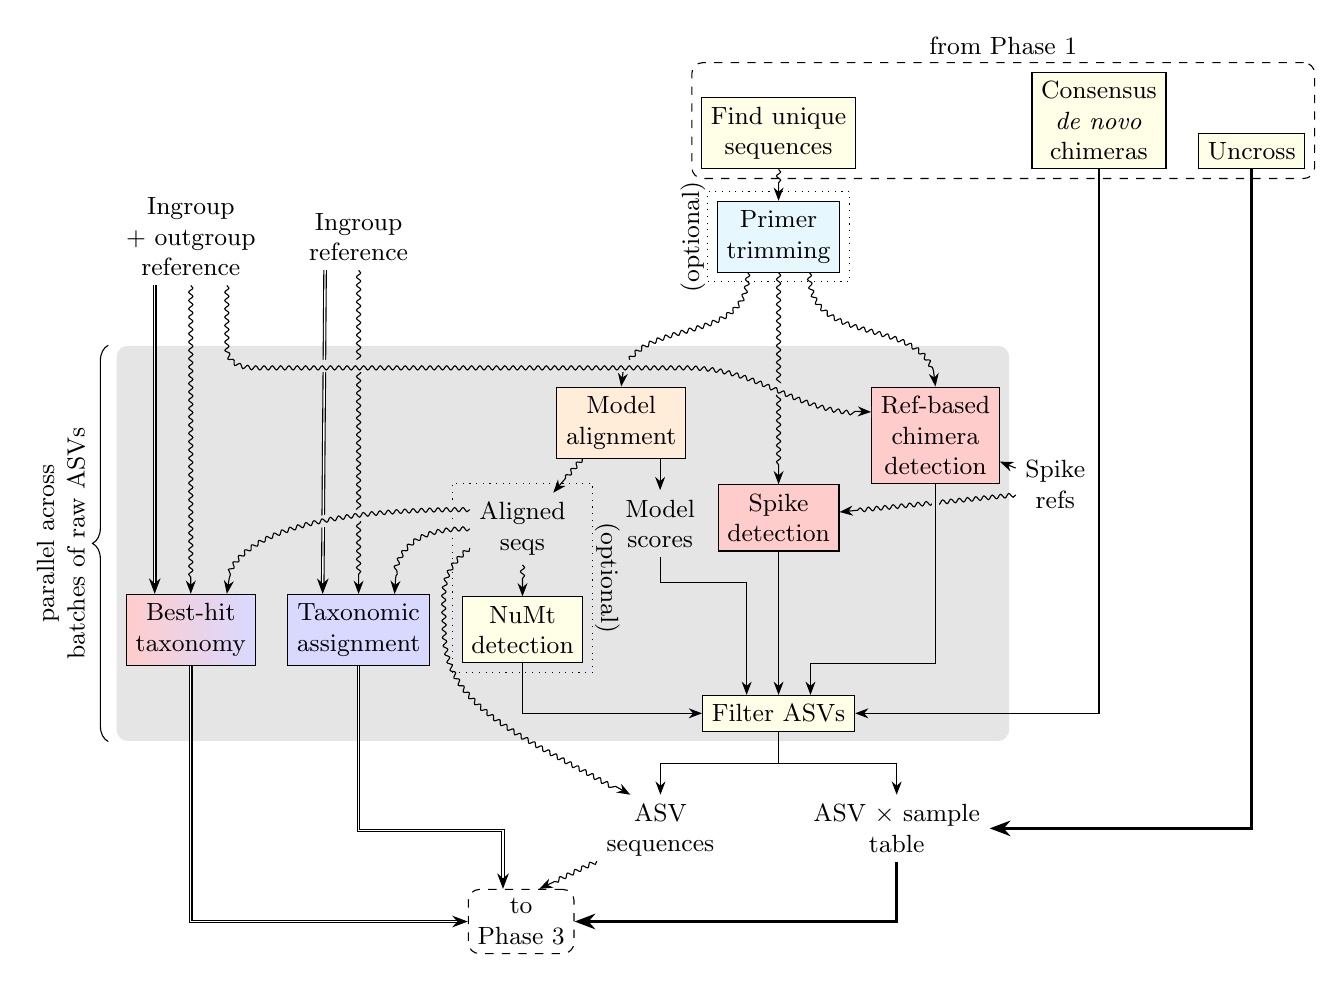
\begin{tikzpicture}[font=\small,node distance=4mm]

\node[vsearch, anchor=north east] (chimera2) {Ref-based \\ chimera \\ detection};
\node[left=of chimera2.south west, vsearch, anchor=north east] (spike) {Spike \\ detection};
\node[left=of $(spike.west|-chimera2.north)$, anchor = north east, infernal] (align) {Model \\ alignment};
\node[below=of $(align.south west)!0.8!(align.south east)$, data] (scores) {Model \\ scores};
\node[below left=of align.south, data, yshift = -1.5mm, xshift = -3mm] (alignment) {Aligned \\ seqs};
\node[below=of alignment, new] (numt) {NuMt \\ detection};
\node[left=of numt, protax] (protax) {Taxonomic \\ assignment};
\node[draw, fit=(numt) (alignment), dotted] (align_opt) {};
\node[right=1mm of align_opt, anchor=base, align=center, rotate=-90] (align_option) {(optional)};


\node[left=of protax, protax_or_vsearch] (besthit) {Best-hit \\ taxonomy};
\node[below=of $(spike |- numt.south)$, new] (asv_filter) {Filter ASVs};

\node[above=40mm of spike, new] (seq_all) {Find unique\\sequences};
\node[below=of seq_all, cutadapt] (trim2) {Primer \\ trimming};
\node[draw, fit=(trim2), dotted] (trim2opt){};
\node[left=1mm of trim2opt, anchor=base, align=center, rotate=90]{(optional)};
\coordinate[above=of $(seq_all |- chimera2.north)$] (p1);

\coordinate (p3) at (seq_all.south east -| chimera2.east);
\node[new, right= of p3, align=center, anchor=south west] (combine) {Consensus \\ \emph{de novo} \\ chimeras};
\node[new, right = of combine.south east, anchor=south west] (uncross) {Uncross};

\node[data] (ingroup_ref) at (protax|-trim2) {Ingroup \\ reference};
\node[data] (outgroup_ref) at (besthit|-trim2) {Ingroup \\ + outgroup \\ reference};
\node[right = 2mm of chimera2.south east, data] (spike_ref) {Spike \\ refs};

\begin{pgfonlayer}{background}
\node[fit = (seq_all) (combine) (uncross), rounded corners, dashed, draw] (phase1) {};
\node[fit = (chimera2) (protax) (align) (p1) (besthit) (asv_filter), parallel] (batch) {};
\end{pgfonlayer}
\draw[decorate, decoration={brace, raise = 1mm, amplitude=2mm}] (batch.south west) -- (batch.north west) ;
\node[rotate=90,left=4mm of batch, anchor=base, align=center] (batch_label) {parallel across \\ batches of raw ASVs};
\coordinate[below= of asv_filter] (p2);
% \node[left=of spike, align=center] (spikecount) {Spike \\ counts};
\node[below right = 4mm and 15mm of p2, data, anchor=north] (ASV) {ASV $\times$ sample \\ table};
\node[below left = 4mm and 15mm of p2, data, anchor=north] (nonspike) {ASV \\ sequences};

\node[above=1mm of phase1.north, anchor=base] {from Phase 1};
\node[draw, dashed, rounded corners, below left=of nonspike, align=center] (phase3) {to \\ Phase 3};

\draw[-Stealth,single reads] (seq_all) -- (trim2);
\draw[-Stealth,single reads] ($(trim2.south west)!0.25!(trim2.south east)$) .. controls +(270:10mm) and +(90:10mm) .. (align.north);
\draw[-Stealth,single reads] (trim2) -- (spike.north);
\draw[-Stealth,single reads] ($(trim2.south west)!0.75!(trim2.south east)$) .. controls +(270:10mm) and +(90:10mm) .. (chimera2.north);

\draw[-Stealth, single reads] (ingroup_ref) -- (protax);
\draw[-Stealth, taxonomy] (ingroup_ref.225) -- (protax.135);
\draw[-Stealth, single reads] (outgroup_ref) -- (besthit);
\draw[-Stealth, taxonomy] (besthit.135|-outgroup_ref.south) -- (besthit.135);

\draw[-Stealth] ($(align.south west)!0.8!(align.south east)$) -- (scores);
\draw[-Stealth,single reads] ($(align.south west)!0.2!(align.south east)$) -- (alignment);
\draw[-Stealth,single reads] (alignment) -- (numt);
\draw[gray!20, line width=1.5mm] (alignment.west) ..controls +(180:5mm) and +(90:7mm) .. (protax.45);
\draw[-Stealth,single reads] (alignment.west) ..controls +(180:5mm) and +(90:7mm) .. (protax.45);
\draw[gray!20, line width=1.5mm] (alignment.160) .. controls +(180:10mm) and +(90:10mm) .. (besthit.45);
\draw[-Stealth,single reads] (alignment.160) .. controls +(180:10mm) and +(90:10mm) .. (besthit.45);
\draw[gray!20, line width=1.5mm] ($(align.north-|besthit.east)!0.5!(besthit.east|-batch.north)$) -- ($(align.north east)!0.5!(align.east|-batch.north)$) .. controls +(0:10mm) and +(180:10mm) .. (chimera2.160);
\draw[-Stealth,single reads] (outgroup_ref.south-|besthit.45) -- (batch.north-|besthit.45) .. controls +(270:2mm) and +(180:2mm) .. ($(align.north-|besthit.east)!0.5!(besthit.east|-batch.north)$) -- ($(align.north east)!0.5!(align.east|-batch.north)$) .. controls +(0:10mm) and +(180:10mm) .. (chimera2.160);
\draw[-Stealth,single reads] (spike_ref.195) -- (spike);
\draw[-Stealth,single reads] (spike_ref) -- (chimera2);
% \draw[-Stealth,single reads] (spike_ref.165) .. controls +(180:10mm) and +(0:10mm) .. ($(chimera2.south east)!0.5!(combine.south-|chimera2.east)$);


\draw[-Stealth] (numt) |- (asv_filter);
\draw[-Stealth] (scores) -- +(0,-7.5mm) -| (asv_filter.150);
\draw[-Stealth] (spike) -- (asv_filter);
\draw[gray!20,line width=1mm] (chimera2) -- (chimera2 |- numt.south);
\draw[-Stealth] (chimera2) -- (chimera2 |- numt.south) -| (asv_filter.30);
\draw[-Stealth] (combine) |- (asv_filter);
% \draw[-Stealth] (spike) -- (spikecount);
\draw[-Stealth] (asv_filter) -- (p2) -| (ASV);
\draw[-Stealth] (p2) -| (nonspike);
% \draw[white, line width=1mm] (uncross|-seqrun.south) |- (ASV);
\draw[-Stealth,table] (uncross) |- (ASV);
\draw[-Stealth, single reads] (alignment.200) .. controls +(220:5mm) and +(90:5mm) .. ($(protax.east)!0.5!(numt.west)$) .. controls +(270:10mm) and +(150:15mm) .. (nonspike.130);

\draw[-Stealth, taxonomy] (besthit) |- (phase3);
\draw[-Stealth, taxonomy] (protax) |- (protax|-nonspike) -| ($(phase3.north west)!0.33!(phase3.north east)$);
\draw[-Stealth, single reads] (nonspike) -- ($(phase3.north west)!0.67!(phase3.north east)$);
\draw[-Stealth, table] (ASV) |- (phase3);

\end{tikzpicture}
